\lvli{D-wave}
\lvlii{Architettura del processore}
\lvliii{Introduzione}
\cite{ACI}Questa sezione andrà a parlare dei primi due computer commerciali della \textit{D-Wave} che sono il \idx{D-Wave One} e il \idx{D-Wave Two} e andrà ad esplorare la loro architettura per comprendere l'idea che la \textit{D-Wave} ha di quantum computer. Il loro computer si basa sul quantum annealing spesso abbreviato con QA. Il processore ha dei qubit sviluppati con l'architettura rf-SQUID che sono degli anelli superconduttivi che possono essere accoppiati a due a due. Un quantum computer per eseguire algoritmi ha necessita di un numero considerevole di qubit, il \textit{D-Wave One} ne possiede 128 mentre il \textit{D-Wave Two} ne possiede 512. Un numerò così grande di qubit genera delle problematiche di costruzione soprattutto per quanto riguarda la scalabilità. Fortunatamente gran parte dell'elettronica dell'epoca fu riutilizzata per sviluppare il primo modello il \textit{D-Wave One} basato sull'architettura dei \idx{SFQ} single flux quanta. Da allora la tecnologia si è evoluta e con nuove tecniche e nuove architetture si è realizzato il \textit{D-Wave Two} computer di seconda generazione. Le innovazioni principali non furono sui qubit o sulla loro gestione di accoppiamento, ma furono sul sistema di controllo del processore e sul sistema di fabbricazione. Il \textit{D-Wave One} usava un demultiplexer per controllare gli SFQ, questo implicava che per controllare $N$ qubit bisognava avere $O(\log{N})$ linee di indirizzamento. Questa architettura era stata studiata per dissipare meno energia possibile durante la programmazione. Il \textit{D-Wave Two} ha invece sradicato completamente il problema, eliminando totalmente la dissipazione di energia statica attraverso l'introduzione dell'\idx{indirizzamento XYZ} con l'utilizzo di solo $O(\sqrt[3]{N})$ linee.
Un altro obiettivo raggiunto del \textit{D-Wave Two} è stato il miglioramento delle prestazioni dell'algoritmo di annealing ottimizzando la scala energetica dei qubit, traguardo raggiunto riducendo la dimensione fisica dei qubit di un fattore di due. Questa modifica ha influito negativamente sul processo di fabbricazione obbligando ad aumentare da quattro a sei il numero dei livelli di metallo, ma positivamente ha aumentato di quattro volte la densità del processore. Ora proseguiamo analizzando la topologia del processore che è comune per entrambe le macchine.

\lvliii{Topologia}
\lvliv{I vincoli}
\cite{ACI}Il processore sul quantum annealing è basato sul modello di Ising e mira a risolvere problemi di minimizzazione sui grafi, in particolare è stato pensato per risolvere questo problema: dato un grafo fisico $G$, minimizzare la seguente forma quadratica di variabili discrete $s_i \in \{-1, +1\}$:
$$E(\vec{s}, \vec{h}, \vec{J}) = \sum_{i \in nodes(G)} h_i s_i + \sum_{<i,j> \in nodes(G)} J_{ij} s_i s_j$$
dati come parametri del problema $h_i, J_{ij} \in \{-1, -7/8, ..., +7/8, +1\}$.
D-wave per risolvere questo problema ha sviluppato una topologia su misura nel \textit{D-Wave One} e nel \textit{D-Wave Two} chiamata \idx{Chimera}.

La struttura Chimera è stata basata su tre \idx{vincoli topografici} importanti: non planarità, possibilità di sviluppare grafi completi e la possibilità di avere dei circuiti di controllo. La \idx{non planarità} è necessaria quando si vuole poter risolvere problemi np-completi; la soluzione è stata ottenuta introducendo la catena di qubit. L'\idx{abilità di sviluppare grafi completi} non è solo legata alla non planarità ma è anche legata alla possibilità di mappare il grafo di qubit logici (software) in qubit fisici (hardware) i quali differiscono in termini di possibilità di interconnessione. Come anticipato in precedenza un qubit logico può essere anche sviluppato con quella che viene chiamata una catena di qubit fisici ma può essere rappresentato da strutture più complesse come alberi o sottografi. Per capire se un grafo può essere rappresentato all'interno dell'hardware si utilizza la \textit{straightforward prescription}. Bisogna quindi disporre di un numero superiore di qubit fisici rispetto a quelli teorici e con l'aumentare del loro numero la necessità di avere dei \idx{circuiti di controllo} diventa indispensabile, infatti sebbene pochi qubit possono essere controllati con precisione da sole linee di controllo, molti qubit presentano dei problemi risolvibili solo mediante un circuito di controllo dedicato. Attualmente il processore QA ha sette \textit{"manopole"} per controllare il sistema, in particolare ce ne sono sei associate ad ogni qubit, necessarie per regolarizzare le variazioni dovute alla fabbricazione e una associata agli accoppiamenti dei qubit stessi. Per realizzare queste manopole di controllo sono stati impiegati dei bias a flusso statico, programmabili da sistemi di controllo che combinano la trasformazione digitale analogica alla scrittura di una memoria persistente. Questi sistemi di controllo sono stati chiamati flux DAC o \idx{$\Phi$-DAC} (flux digital analog converter). Il loro numero considerevole all'interno del circuito influenza la forma dei qubit e la topologia del circuito.

Oltre ai vincoli della topologia ci sono anche altre costrizioni, in particolare andremmo ad esporne le cinque più importanti. Dal punto di vista ideale ogni qubit dovrebbe essere connesso ad ogni altro; sfortunatamente al livello fisico c'è una limitazione di \idx{interconnessione tra qubit} perché nonostante si possano realizzare catene, alberi, e sottografi dei qubit logici, un qubit può essere collegato solo ad un numero di qubit minore di $10$ a causa di caratteristiche non ideali e problemi delle scale energetiche introdotti dal superamento di questo limite. Un altro vincolo che deriva dal minimizzare le scale di energia è la \idx{minimizzazione del disaccoppiamento} ovvero minimizzare la superficie dei qubit che non viene utilizzata per gli accoppiamenti con altri qubit. Idealmente tutta la superfice dei qubit dovrebbe essere intersecata dalla superfice dei sistemi di accoppiamento e tutti i sistemi di accoppiamento dovrebbero avere la superfice intersecata con i qubit. Lavorare a bassi livelli di energia comporta anche una particolare \idx{attenzione ai rumori} esterni ed a rumori dovuti ad accoppiamenti indesiderati con altre parti del circuito. Questa struttura composta da qubit, sistemi di accoppiamento e $\Phi$-DAC è implementata su un chip ovvero utilizza un'\idx{integrazione bidimensionale}. Sebbene sviluppare questa tecnologia attraverso un'integrazione tridimensionale sarebbe dal lato teorico più vantaggiosa, dal lato pratico è molto più semplice sviluppare attraverso un sistema scalabile a due dimensioni. Qui si introduce il quinto dei nostri vincoli, ovvero, l'introduzione della \idx{unità piastrella}. Proprio come accade nella realtà quotidiana, ricoprire un pavimento con piastrelle regolari è molto più facile che farlo con oggetti non regolari, questa comodità si percepisce sempre di più aumentando la superfice che vogliamo ricoprire.

\lvliv{Le soluzioni di Chimera}
\begin{wrapfloat}{figure}{I}{0pt}
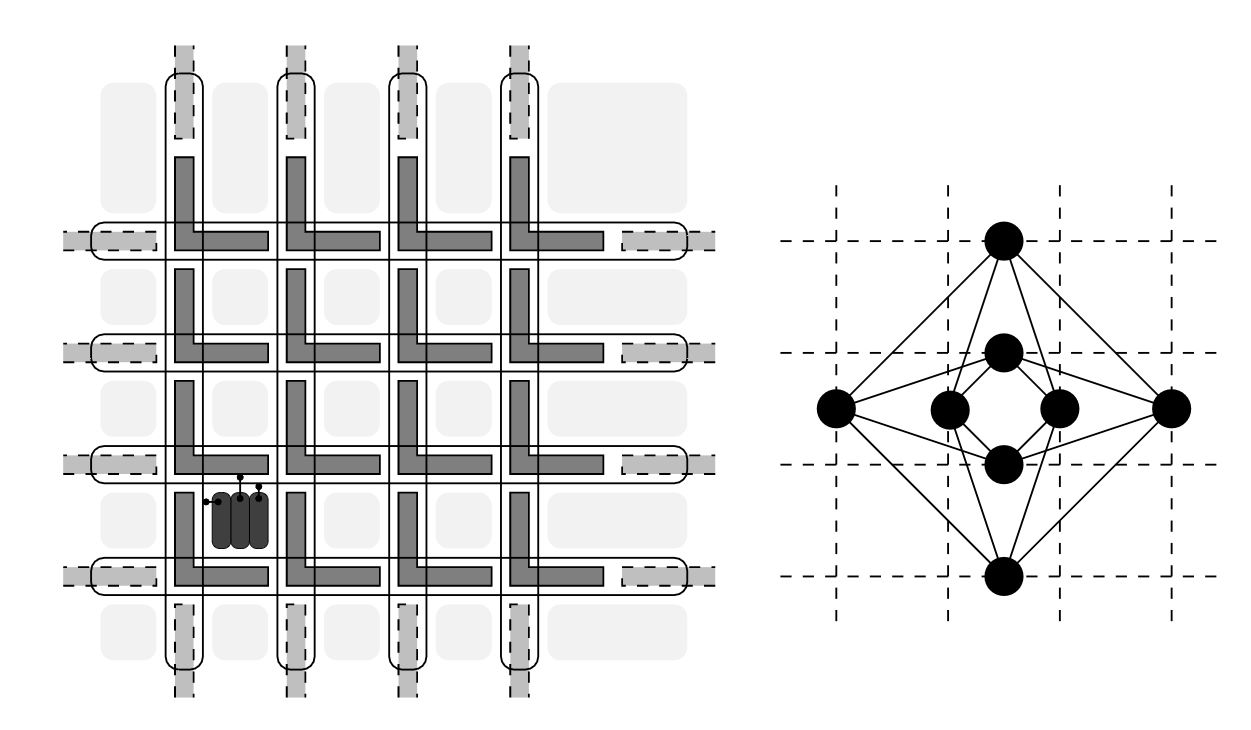
\includegraphics[width=0.4\textwidth]{Immagini/chimera.jpg}
\caption{Topologia chimera.}
\label{figura:chimera}
\end{wrapfloat}
\cite{ACI}La scelta della struttura Chimera è risultata vantaggiosa per risolvere molti di questi problemi. La prima caratteristica importante, che ha questa struttura, è l'utilizzo dei flux qubit. Questi qubit a flusso sono degli anelli macroscopici con delle interruzioni chiamate \textit{Josephson junction}.

La \idx{Josephson Junction}\cite{JJQ} è una giunzione tra due superconduttori, che hanno un accoppiamento debole, uniti attraverso un sottile strato isolate che svolge il ruolo di barriera di potenziale. Ci sono vari modi per realizzare una giunzione Josephson, abbiamo due categorie principali per i metalli distinte in base alle temperature utilizzate: per le temperature basse \idx{LTS} (Low Temperature Superconductors) oppure per gli ossidi a temperature elevate \idx{HTS} (High Temperature Superconductors). Per l'elettronica LTS le giunzioni ad effetto tunnel svolgono un ruolo molto importante grazie alla loro bassa dissipazione di energia. In particolare sono delle buone candidate per la costruzione dei qubit per le loro proprietà non lineari.

La loro struttura macroscopica permette di deformare il corpo del qubit allungandolo e ruotandolo a piacere a seconda delle necessità. Quasi allo stesso modo vale per i sistemi di accoppiamento. Una unità piastrella Chimera è composta da otto qubit, quattro orizzontali e quattro verticali disposti a griglia ed accoppiati nelle loro intersezioni. L'unità è strutturata in modo che disponendo due piastrelle adiacenti, sia in orizzontale che in verticale, si possano allineare i qubit e quindi anche supportare accoppiamenti tra qubit interni e qubit esterni alla piastrella. Questa disposizione di qubit è associabile ad un grafo non planare, ovvero ad un grafo che disteso su un piano non può essere disegnato senza incrociare gli archi.
Usando l'abilità di creare catene di qubit fisici, esiste un approccio diretto per incorporare grafici completi fino a $4N$ nodi in una griglia $N \times N$ formata da piastrelle $K_M$ composte da $M + M$ qubit. Questa griglia viene indicata con $C_N$. Nel \textit{D-Wave One} la griglia è formata da $4\times4$ piastrelle quindi un $C_4$ mentre nel \textit{D-Wave Two} è formata da un $8\times8$ ovvero un $C_8$, entrambe con una piastrella $K_4$. Un modo pratico per vedere questo grafo completo è prendere una piastrella $K_4$ e decidere di rappresentare un qubit logico come due qubit fisici, in particolare scegliamo di prenderne uno orizzontale e uno verticale. Così facendo avremo quattro qubit totali rappresentabili all'interno della cella dove ogni qubit si collega con tutti gli altri tre formando un grafo completo. Diventa intuitivo poi generalizzare questo concetto allungando la nostra catena di quibit fisici attraverso più piastrelle. Un'altra caratteristica della struttura Chimera è la possibilità di avere integrati i sistemi di controllo sulla piastrella. Ogni buco della griglia $4\times4$ è occupato da tre sistemi di controllo: uno per controllare il qubit verticale, uno per controllare il qubit orizzontale e uno per controllare il loro sistema di accoppiamento. I sistemi di accoppiamento hanno una forma a L che si distribuisce, partendo dal punto in cui i qubit si sovrappongono, per tutti e due i qubit fino a poco prima del prossimo incrocio con altri qubit. Questa forma permette la massima copertura reciproca di superfici tra sistema di accoppiamento e qubit.
La regolarità della piastrella Chimara consente la massima scalabilità del circuito lasciando come vincoli il numero di linee indirizzabili e quelli strettamente legati alla fabbricazione. La scelta di avere un $K_4$ è dipende da due fattori importanti. Il primo è legato al fatto che $\Phi$-DAC hanno una disposizione ottimale in una gliglia $5\times5$ che si sovrappone alla griglia $4\times4$ dei qubit riducendo al minimo lo spreco di spazi. Il secondo è che il numero di $\Phi$-DAC usati per bilanciare le variazioni di produzione e il numero di $\Phi$-DAC usati effettivamente per la risoluzione del problema, si equiparano.

\lvliii{$\Phi$-DAC}
\lvliv{$\Phi$-DAC teorici}
\begin{wrapfloat}{figure}{I}{0pt}
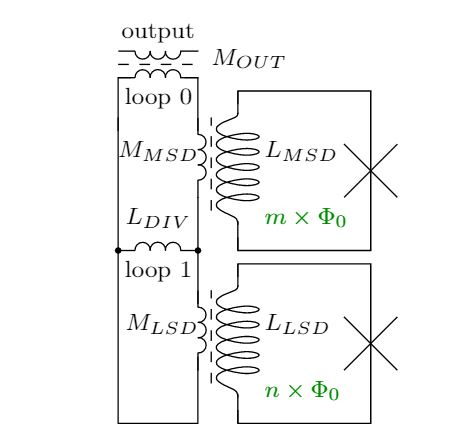
\includegraphics[width=0.4\textwidth]{Immagini/fluxdac-logico.jpg}
\caption{Circuito logico flux-dac.}
\label{figura:fluxdac-logico}
\end{wrapfloat}
\cite{ACI}I $\Phi$-DAC sono i diretti responsabili della precisione del sistema. La capacità di flusso di ogni singolo $\Phi$-DAC è regolata da 8 bit di range dinamico. Per massimizzare questo range dinamico e per minimizzare l'area occupata è stato scelto di implementare la maggior parte dei $\Phi$-DAC come dispositivi a doppio stage. Ogni $\Phi$-DAC è composto da due SQUID dove ognuno di questi SQUID serve a rappresentare una cifra, la più significativa è chiamata \idx{MSD} (most significant digit) mentre quella meno significativa è chiamata \idx{LSD} (less significant digit). In uno SQUID può essere memorizzato, attraverso impulsi SFQ, una cifra di flusso quantistico $m$ che può variare in $-8 \le m \le +8$.

La parola \idx{SQUID}\cite{SQD} è un acronimo che sta per \textit{Superconducting Quantum Interference Devices} ovver per dispositivo ad interferenza quantistica superconduttivo. Sono dispositivi che che servono a misurare il flusso magnetico ed per indicarne il valore madano in output un voltaggio. Lo SQUID è un anello superconduttivo con una o più giunzioni Josephson.

Oltre agli SQUID nei $\Phi$-DAC è presente una scala di due anelli connessi sia agli SQUID che all'output attraveso delle induttanze.
Il primo anello ($loop_0$) comprende tre induttanze $M_{MSD}$ per collegarsi allo SQUID MSD attraverso $L_{MSD}$, $M_{OUT}$ per collegarsi verso il dispositivo di lettura che può essere un qubit piuttosto che un sistema di accoppiamento e $L_{DIV}$ in comune con il secondo anello ($loop_1$) che in aggiunta ha $M_{LSD}$ per collegarsi allo SQUID LSD attraverso $L_{LSD}$. L'induttanza $L_{DIV}$ serve a scalare il segnale entrante dalla cifra meno significativa.
Un SFQ $\phi_0$ aggiunto allo SQUID MSD viene scritto sul primo anello attraverso il rapporto delle loro induttanze $\frac{M_{MSD}}{L_{MSD}}\Phi_0$.
Lo stesso segnale verrà mandato in output come
$$\hat{\Phi}_0 = \frac{M_{MSD}}{L_{MSD}}\frac{M_{tot0}}{M_{OUT}}\Phi_0$$
dove $M_{tot0}$ è l'induttanza totale del primo anello $M_{tot0} = M_{OUT} + M_{MSD} + M_{DIV}$. Dalle formule sopra citate possiamo notare che il flusso in uscita aumenta in modo lineare con il numero di SFQ aggiunti o sottratti dagli SQUID. In realtà esisterebbe anche una componente non lineare, che non viene tenuta conto perché nel caso della \textit{D-Wave} è trascurabile, essendo le dimensioni delle induttanze molto inferiori degli SQUID.
Un SFQ $\phi_0$ aggiunto allo SQUID $L_{LSD}$ viene scritto sulla scala come
$$\hat{\Phi}_0 = \frac{M_{LSD}}{L_{LSD}}\frac{L_{DIV}}{L_{tot1}}\Phi_0$$
dove $M_{tot1} = M_{DIV} + M_{LSD}$. Ognuno dei due SQUID può memorizzare 8 SFQ sia in un verso che nell'altro per un totale di 16 valori rappresentabili con l'equivalente di $\log_2{16} = 4$ bit. Il LSD è fatto in modo da suddividere ogni step del MSD in altri 16 step. $\Phi$-DAC è quindi equivalente ad un dispositivo a $4_{MSD} + 4_{LSD} = 8$ bit con $2^8 = 256$ valori rappresentabili.
La scelta di usare al massimo 256 valori dipende dai limiti della tecnologia attuale che limita il numero di bit a causa delle tolleranze di errore di produzione che possono portare i valori fuori dai loro margini.

\lvliv{$\Phi$-DAC fisici}
\begin{wrapfloat}{figure}{I}{0pt}
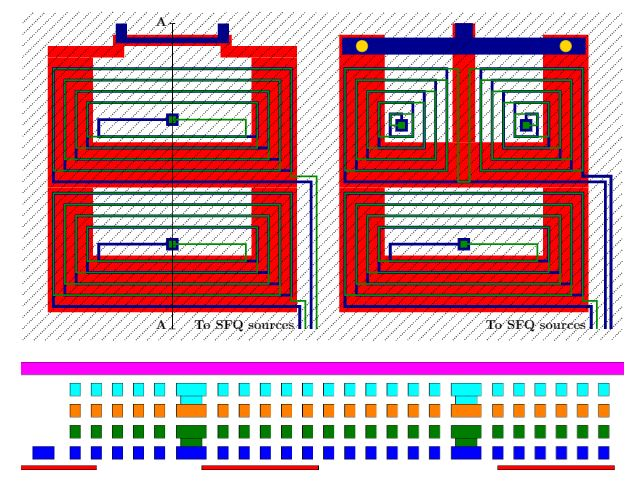
\includegraphics[width=0.4\textwidth]{Immagini/fluxdac-fisico.jpg}
\caption{Circuito fisico flux-dac.}
\label{figura:fluxdac-fisico}
\end{wrapfloat}
\cite{ACI}Ora che abbiamo visto i $\Phi$-DAC da un punto di vista logico possiamo passare ad analizzare un modello più reale. Nel modello reale il $\Phi$-DAC è realizzato su 6 livelli. Il livello più basso è occupato dalla scala induttiva che è costituita da due rondelle galvanicamente collegate assieme. I quattro livelli successivi sono occupati dalle spirali degli SQUID che si sovrappongono a gruppi di due ai due fori del livello inferiore. L'ultimo livello composto da uno scudo \textit{sky-plate} è utilizzato come schermatura che serve per ridurre accoppiamenti indesiderati tra i $\Phi$-DAC e le altre componenti del circuito. Il collegamento tra $\Phi$-DAC e dispositivo in uscita avviene nel secondo livello attraverso un \textit{microstrip transformer}. Sfortunantamente non tutti i $\Phi$-DAC hanno la stessa forma. Hanno una struttura diversa ad esempio quelli che controllano le giunzioni \textit{Josephson junction composte} \idx{CJJ} di cui fanno parte i sistemi di accoppiamento, i sintonizzatori di induttanza e i compensatori di corrente persistenti, che necessitano di poter usufruire di maggiore sensibilità ovvero di variazioni di flusso pari a metà $\Phi_0$. Per aumentare tale controllo si è unito l'anello del CJJ del dispositivo di output con il primo anello della scala induttiva. Un'ulteriore complicazione di questa particolare struttura è che il secondo anello deve essere accoppiato con una forza uguale ad entrambe le metà del CJJ di destinazione, per evitare l'accoppiamento nel corpo del dispositivo. Per ottenere questo traguardo il secondo anello è stato diviso in due metà, modificando di conseguenza i quattro livelli di spirale sovrapposti in quella zona per mantenerne il massimo accostamento.

Come abbiamo visto in questo ultimo passaggio il modello teorico si distanzia sempre di più da quello reale. Altre differenze sono nella trasmissione del segnale. Il secondo anello fluisce direttamente nel primo il quale può raggiungere l'uscita non solo attraverso la scala induttiva ma anche attraverso la connessione magnetica. Il flusso delle spire dello SQUID $L_{MSD}$ raggiunge direttamente l'uscita con senso opposto a quello passante per il primo anello generando interferenza.

\lvliv{Generatori di SFQ}
\begin{wrapfloat}{figure}{I}{0pt}
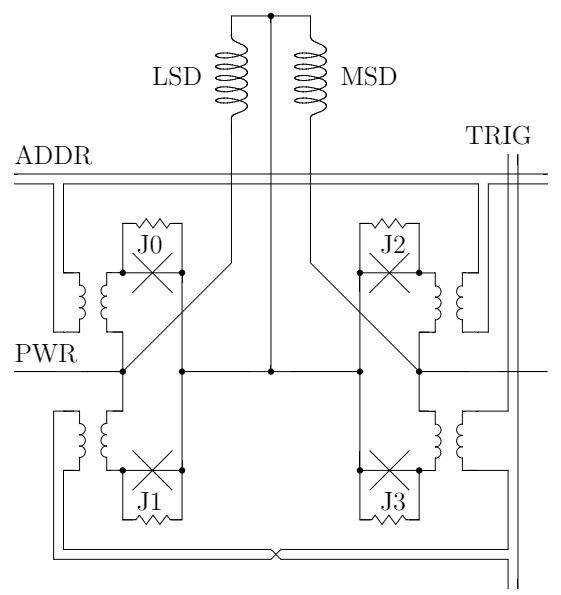
\includegraphics[width=0.4\textwidth]{Immagini/sfq.jpg}
\caption{Circuito logico single flux quanta.}
\label{figura:sfq}
\end{wrapfloat}
\cite{ACI}Fino ad ora abbiamo trattato il \idx{generatore di SFQ} come un semplice generatore di corrente ma in realtà è un oggetto molto più complesso, ora vedremo come è strutturato. Ogni generatore di SFQ è formato da due \idx{DC-SQUID} (Direct Current SQUID) uno per MSD e uno per LSD. Un DC-SQUID è un anello superconduttivo a doppia giunzione \textit{Josephson junction}. Chiamiamo le due giunzioni $J0$ e $J1$ per LSD e $J2$ e $J3$ per MSD. Ogni anello è collegato in maniera diretta con l'alimentazione $PWR$ e con la propria induttanza $L_{MSD}, L_{LSD}$. In ogni anello ci sono anche due resistenze ognuna in parallelo ad una giunzione, e due induttanze per collegarsi a due linee, quella degli indirizzi $ADDR$ e quella di trigger $TRIG$. In particolare la linea di $TRIG$ dell'anello LSD è invertita rispetto a quello dell'anello MSD. Per eseguire un'operazione di scrittura la procedura è la seguente. Prima si accende $PWR$ creando una corrente di bias di circa $\frac{I_c}{2}$. Successivamente si abilita $ADDR$ che aggiunge un flusso di bias al corpo dello SQUID. Si prosegue abilitando $TRIG$ in maniera che sia additivo per l'anello LSD, introducendo corrente sufficiente fino a che $J0$ non supera il suo punto critico, generando un cambiamento di fase di $2\pi$ con conseguente produzione di un SFQ.
In fine, si decrementa $TRIG$ causando il cambiamento di fase di $J1$ che riporta lo SQUID al suo stato di flusso base. Sapendo che l'induttanza $L_{LSD}$ è maggiore dell'induttanza dello SQUID, questo ciclo di scrittura viene ripetuto più volte per assicurarsi che la corrente scritta nell'anello di memorizzazione sia comparabile a quella di $PWR$. Due cose da notare in questo procedimento sono l'utilizzo di $PWR$ e quello di $TRIG$ e $ADDR$. Il segno di $PWR$ corrispone anche al segno del SFQ, se $PWR$ è negativo il SFQ andrà sottratto. La scrittura avviene solo se tutti e tre i segnali sono attivi, in particolare se $ADDR$ e $TRIG$ hanno lo stesso verso. Essendo invertito $TRIG$ tra i due anelli LSD e MSD quando è concorde al verso di LSD è discorde a quello di MSD disabilitando MSD. Le tre linee $PWR$, $TRIG$ e $ADDR$ compongono il sistema di indirizzamento XYZ anticipato precedentemente con un numero di linee pari a $O(\sqrt[3]{N})$ per $N$ $\Phi$-DAC.
La stabilità del $\Phi$-DAC è completamente determinata da due parametri $\Phi_b$ somma dei flussi di bias di $TRIG$ e $ADDR$ $$\Phi_b = ADDR + TRIG$$
e $I_b$ somma delle corrente circolante di $PWR$ e quella dipendente dallo stato
$$I_b = I_{PWR} -n \Delta I_{sfq}$$
Queste due variabili possono essere viste come coordinate di uno spazio bidimensionale $(\Phi_b, I_b)$ in cui poter disegnare i confini di stabilità dove il flusso è persistente. In questo spazio si possono identificare due tipi di regione d'interesse: quelle attive e quelle proibite. I valori delle tre linee sono scelti in modo da massimizzare le regioni attive, dove la transizione rispetta i criteri, e minimizzare le zone proibite, dove i criteri non sono rispettati.

\lvliv{$\Phi$-DAC reset}
\cite{ACI}Le operazioni viste fino ad ora sono delle variazioni che dipendono da uno stato di partenza, questo implica che è necessaria un'operazione in grado di portare il $\Phi$-DAC da un qualsiasi stato ad uno stato a noi noto. Lo stato di partenza scelto è $I_{PWR} = 0$ e questa operazione è stata nominata reset. Per applicare un reset al $\Phi$-DAC bisogna generare un flusso con ampiezza superiore alle soglie di zona attiva di $\Phi_b$ fino a quando il $\Phi$-DAC non raggiunge il suo livello di energia di minimo corrispondente a zero SFQ. La tecnologia dei \textit{D-Wave One} e nel \textit{D-Wave Two} prevede il reset simultaneo per tutti i $\Phi$-DAC.

\lvliv{Dimensionamento del $\Phi$-DAC}
Come esaminato in precedenza le dimensioni del $\Phi$-DAC sono quelle che regolano le dimensioni dei qubit, delle loro scale energetiche e quindi delle prestazioni degli algoritmi. Minimizzare l'area è quindi di vitale importanza. D'altro canto dei buoni $\Phi$-DAC devono avere come caratteristiche un'ampia scala di valori programmabili e una buona precisione, proprietà che migliorano con l'aumentare dell'area e in proporzione al prodotto $L \times I_c$ dove $L$ è l'induttanza dell'anello di memorizzazione e $I_c$ è la corrente per generare un SFQ. Tenendo fissa l'area del $\Phi$-DAC, con l'intento di massimizzare il prodotto $L \times I_c$, si sviluppa un trade-off tra le due caratteristiche sopra elencate, dimensione dell'induttanza $L$ e dimensione degli SQUID $I_c$. Considerando $L$ come $\alpha x$, proporzionale all'area rispetto ad una costante alpha, e $I_c = J_c (1-x)$ dove $J_c$ è la densità di corrente, possiamo scrivere:
$$ L \times I_c = \alpha x \times J_c (1-x) \approx x \times (1 - x)$$
Appare lampante che la soluzione ottimale è $x = 0.5$. Questa è la scelta portata avanti nelle tecnologie del \textit{D-Wave One} e del \textit{D-Wave Two}.

\lvlii{Annealing}
\lvliii{Classical annealing}
\begin{wrapfloat}{figure}{I}{0pt}
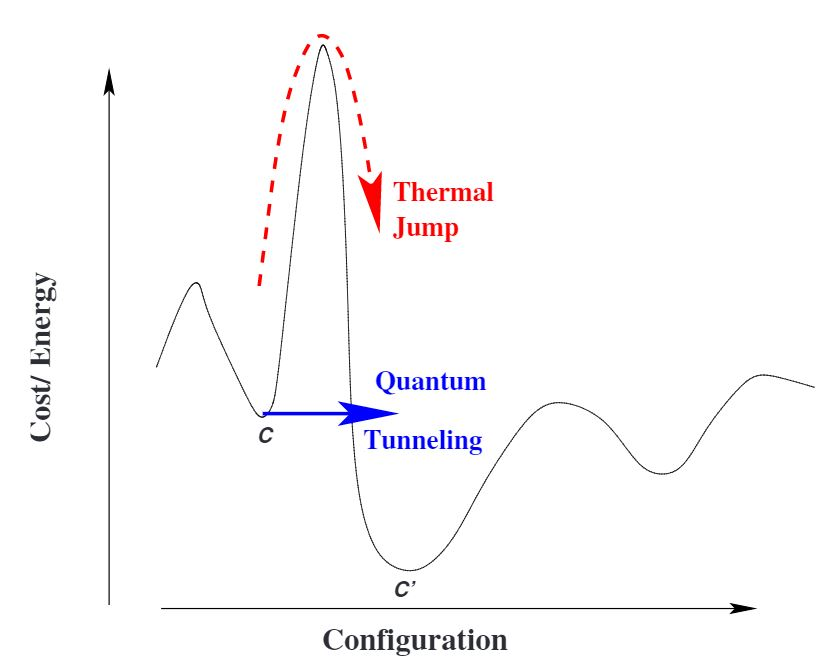
\includegraphics[width=0.4\textwidth]{Immagini/qa.jpg}
\caption{Classical e Quantum annealing.}
\label{figura:qa}
\end{wrapfloat}
\cite{QA,QVC,ST}Il classical annealing \idx{CA} nasce più di 6000 anni fa ed è il più antico metodo di ottimizzazione; veniva utilizzato dai fabbri con l'intento di ridurre lo stress dai metalli. Durante tale processo il metallo viene riscaldato ad alte temperature fino a che non supera la temperatura di austenitizzazione, dopodiché viene gradualmente raffreddato.
Dal punto di vista statistico, quando il metallo si trova nella prima parte del processo i suoi atomi sono disposti in maniera casuale e disordinata e, perciò, l’energia del sistema risulta elevata. Al contrario, allo stato fondamentale (o \textit{ground state}) del solido corrisponde una struttura cristallina con energia di sistema minima.
Abbassamenti troppo bruschi della temperatura possono portare a dei difetti nella struttura del reticolo cristallino impedendo al solido di raggiungere l’energia minima di sistema e quindi la stabilità, detto in altre parole lo stress termico comporta la meta-stabilità del metallo. L’abbassamento graduale usato nell’annealing serve per evitare questo fenomeno e portare il metallo ad una struttura globalmente ottima e stabile. Infatti, il ground state è raggiungibile solo se il valore massimo della temperatura è sufficientemente alto e il raffreddamento è abbastanza lento.

\lvliii{Quantum annealing}
\cite{QVC,QAS}Il quantum annealing come il CA è un metodo di ottimizzazione che mira a raggiungere il ground state. A differenza del CA che usa eccitazioni termiche per saltare sopra le barriere di potenziale, per evitare di rimanere bloccato in un minimo locale, il QA utilizza l'effetto tunnel per passarci attraverso. Il QA risulta vantaggioso più le barriere di potenziale sono alte e strette.

La D-Wave utilizza nel suo computer il QA attraverso il modello di Ising che viene implementato da un network di qubit mediante l'architettura Chimera. Il modello di Ising serve per rappresentare quello che viene chiamato \idx{spin glass} ovvero un magnete disordinato dove il disordine deriva dalla configurazione casuale di allineamento rispetto al nord o al sud magnetico degli atomi in esso contenuti. Il termine \idx{glass} è un'analogia tra il disordine degli spin e il disordine della struttura chimica del vetro.

\lvliii{Funzionamento}
\begin{wrapfloat}{figure}{I}{0pt}
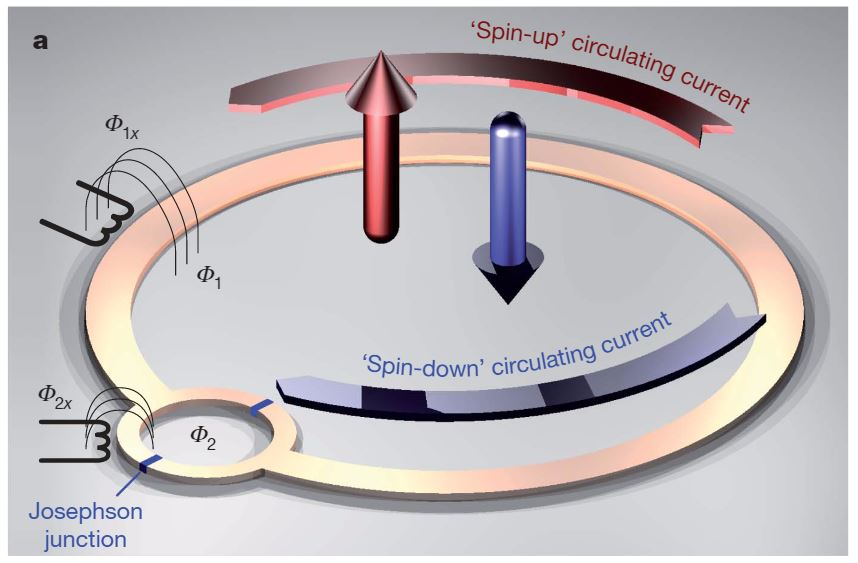
\includegraphics[width=0.4\textwidth]{Immagini/qubit.jpg}
\caption{Qubit.}
\label{figura:qubit}
\end{wrapfloat}
\cite{QAS,QVC}Per crare un processore che sfrutti il quantum annealing si ha bisogno di un sistema quantistico che permetta di programmare i singoli spin e i loro accoppiamenti, eseguire l'annealing quantistico e determinare lo stato di ogni spin. L'idea della D-Wave è stata di utilizzare strutture macroscopiche come le \textit{Josephson junction} per ottenere gli effetti quantistici. Questa è stata la chiave di successo che è riuscita a garantire la programmabilità dei singoli spin su processori che condengono svariati centinaia di qubit.

Un \idx{qubit} è realizzato con l'unione di due anelli uno più grande che chiameremo $a_1$ e uno più piccolo $a_2$. L'anello più piccolo vanta di due \textit{Josephson junction}. Ogni anello è influenzato da un flusso magnetico esterno, rispettivamente $\phi_{x1}$ e $\phi_{x2}$. Il qubit così strutturato non è altro che quello che viene chiamato in meccanica quantistia un pozzo a doppio potenziale. Il pozzo ha come energia di sistema $\phi_1$ e altezza di potenziale $\delta U$ che è controllata tramite $\phi_{2x}$, mentre la distanza $2h$ tra i due minimi di energia è controllata da $\phi_{1x}$.
Questo sistema è possibile modellizzarlo tramite Ising per temperature molto basse dove il verso di rotazione orario o antiorario della circolazione di corrente nell'anello $a_1$ corrisponde al verso del flusso $\phi_1$, calcolato mediante la regola della mano destra, che viene indicato $\left|\uparrow \right\rangle$ e $\left|\downarrow \right\rangle$, o più comodamente $|1 \rangle$ e $|0 \rangle$.
\begin{wrapfloat}{figure}{I}{0pt}
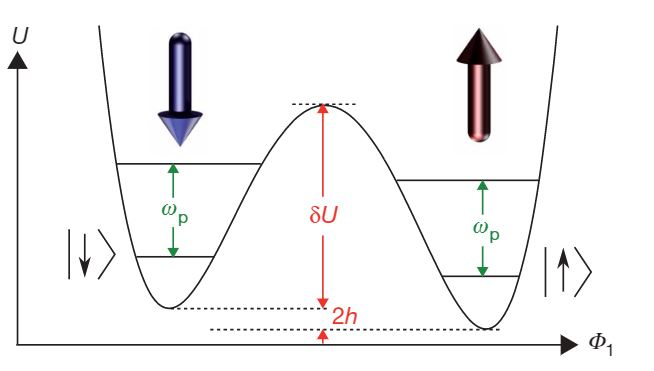
\includegraphics[width=0.4\textwidth]{Immagini/pozzo.jpg}
\caption{Doppio pozzo di potenziale.}
\label{figura:pozzo}
\end{wrapfloat}

La \idx{programmazione dei singoli} spin avviene attraverso il controllo di accoppiamento tra due spin adiacenti tramite i flussi magnetici $\phi_{x1}$ e $\phi_{x2}$ che imporranno un comportamento ferromagnetico o antiferromagnedico per favorire il loro allineamento piuttosto che l'antiallineamento.
Il comportamento di ogni singolo spin viene descritto attraverso l'hamiltoniana del sistema del modello di Ising:
$$H_p = \sum_{i=1}^N h_i \sigma_i^z + \sum_{i,j=1}^N J_{ij} \sigma_i^z \sigma_j^z$$
dove $\sigma_i^z$ e $\sigma_j^z$ sono le matrici di Pauli, rispetto l'asse $z$, aventi come autovettori $\{|1\rangle, |0\rangle\}$. L'architettura hardware permette di programmare in maniera indipendente l'energia di flusso $h_i$ applicata al singolo spin $i$ e l'energia di accoppiamentro $J_{ij}$ tra i due spin $i$ e $j$.

Per \idx{eseguire il QA} in un sistema di spin glass si utilizza il modello di ising trasverso. A differenza del modello tradizionale esso presenta una componente cinetica aggiuntiva trasversa. All'inizio di tale processo il campo magnetico trasverso è molto più grande del legame di accoppiamento tra i singoli qubit. Il sistema viene quindi posizionato in uno ground state rispetto il campo trasverso. Se il campo trasverso viene abbassato in maniera sufficentemente lenta, quando il campo sarà azzerato, il sistema rimmarrà nel ground state anche rispetto alle forze di accoppiamentro tra i qubit. Tale dinamica può essere descritta dalla funzione hamiltoniana:
$$H(t) = \Gamma(t) \sum_{i=1}^N \Delta_i \sigma_i^x + \Lambda(t) H_p$$
$\Gamma$ e $\Lambda$ sono due variabili che rappresentano la dinamica del sistema. $\Gamma$ si attenua $1 \to 0$ contemporaneamente a $\Lambda$ che si amplifica $0 \to 1$ generando un passaggio dolce tra le due componenti. La prima delle due componenti è $\sum_{i=1}^N \Delta_i \sigma_i^x$ esprime lo stato iniziale del sistema dove gli spin sono preparati in uno ground state rispetto ad $x$ e quindi in superposition rispetto ad $z$ con $\Delta_i$ parametro di tunnelling tra $|1\rangle$ e $|0\rangle$. La seconda componete $H_p$ è invece l'hamiltoniana del nostro modello di Ising nel quale ci interessa conoscere le posizioni finali $\sigma_i^z$.

\lvliii{Stabilire il tipo di annealing}
\cite{QAS}Il sistema qui trattato ha bisogno, per funzionare in maniera corretta, di un annealing quantistico e non di una annealing termico.

Se la fluttuazione termica è dominante, il sistema per spostarsi da un minimo locale tramite un salto termico, necessita di un'energia proporzionale a $e^{-\frac{\delta U}{k_B T}}$ dove $T$ è la temperatura e $k_B$ è la costante di Boltzmann.
Quando la barriera supera l'energia fornita al sistema, ovvero quando $\delta U >> k_B T$ esso non potrà più uscire dal minimo locale. Sapendo che $\delta U$ si incrementa con il tempo, possiamo definire un tempo di blocco del sistema $t_{freeze}^{CA}$ dove $\delta U(t_{freeze}^{CA}) \approx k_BT$. Nell'intervallo di tempo in questione, essendo $\delta U$ quasi lineare rispetto al tempo, comporta $t_{freeze}^{CA}$ ad essere linearmente dipendente dalla temperatura $T$.

Diversamente se la fluttuazione quantistica è dominante sarà l'effetto tunnel a diminuire con l'alzarsi della barriera $\delta U$. Ci sarà questa volta un altro tempo $t_{freeze}^{QA}$ che avrà una dipendenza dalla temperatura inferiore a quella di $t_{freeze}^{CA}$. Misurando la dipendenza di $t_{freeze}$ da $T$ possiamo determinare qual'è la componente dominante nell'annealing.

D-wave ha realizzato un esperimento su misura per determinare il tipo di fluttuazione dominante all'interno di un singolo qubit. Si parte cercando di determinare il tempo $t_{freeze}$ nel sistema di spin. Per far ciò si vuol misurare la risposta al gradino del sistema a cambiamenti rapidi della distanza $2h$ tra i due minimi di energia, rispetto alle grandezze di migrazione $\Gamma$ e $\Lambda$.
Dopo un intervallo di tempo $t_d$ si varierà la funzione $h(t)$ da $0 \to h_t$ e si misurerà la probabilità $P_1$ di trovare il sistema nello stato di minimo $|1\rangle$. Le dinamiche che si ottengono sono due a seconda che $h$ sia fatta variare presto o tardi nella scala dei tempi rispetto a $t_{freeze}$.
Se $h$ viene fatto variare presto, quando $\delta U$ è ancora bassa, la probabilità misurata sarà $P_1 \ge 0.5$. In questo caso l'effetto termico sarà dominante e il risultato dipenderà dalla distribuzione di Boltzmann. Invece se $h$ viene fatta variare dopo che la barriera è sufficentemente alta $t_d > t_{freeze}$ il sistema si troverà in uno stato di superposition e la probabilità varrà $P_1 \approx 0.5$. L'istante in cui questa probabilità passerà da $P_1 \ge 0.5$ a $P_1 \approx 0.5$ sarà il nostro $t_{freeze}$.
Facendo variare la temperatura $T$ e misurando il tempo $t_{freeze}$ si rileva una saturazione di $t_{freeze}$ sotto una certa temperatura che chiameremo $T_{threshold}$. Poiché la probabilità $P_1$ non satura a $T_{threshold}$ dove $t_{freeze}$ satura, è un chiaro indicatore che la saturazione di $t_{freeze}$ non dipende dalla saturazione della temperatura $T$ del qubit. La conclusione è che il sistema diventa di tipo quantomeccanico per temperature molto basse sotto una certa soglia $T_{threshold}$ che nei computer della D-wave corrisponde a $45 [mK]$.
\begin{figure}[htbp]
\centering
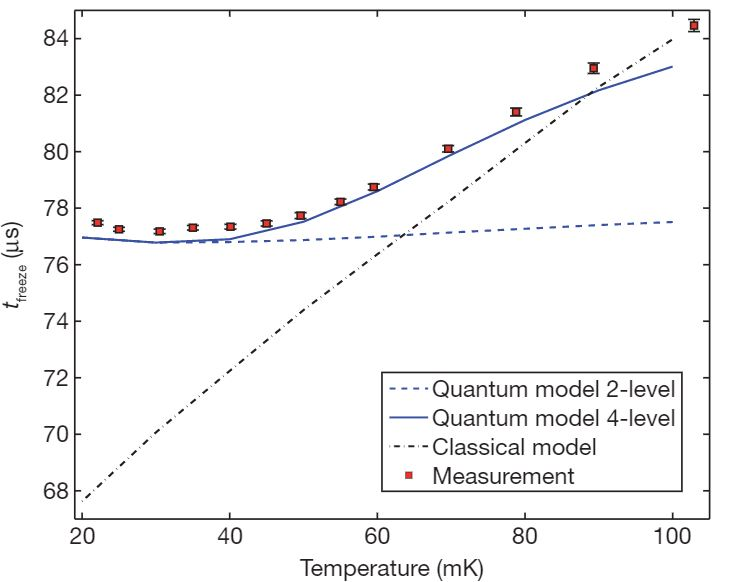
\includegraphics[scale=0.6]{Immagini/qa-qubit.jpg}
\caption{Risultati simulazioni per un singolo qubit.}
\label{figura:qa-qubit}
\end{figure}

\begin{wrapfloat}{figure}{I}{0pt}
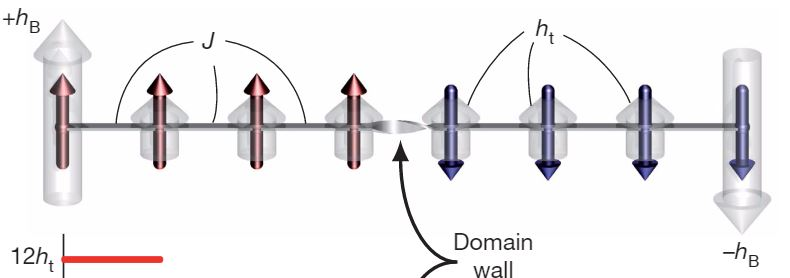
\includegraphics[width=0.4\textwidth]{Immagini/wall.jpg}
\caption{Domain wall.}
\label{figura:wall}
\end{wrapfloat}
Successivamente D-wave ha realizzato un'altro esperimento per dimostrare che la fluttuazione dominante rimane quantistica all'interno di una catena di qubit. L'obiettivo è sempre quello di determinare la dipendenza di $t_{freeze}$ da $T$ sfruttando un calcolo di probabilità sul \idx{domain wall}, ovvero una rottura spontanea della simmetria di un dominio discreto. Ad esempio $|11110000\rangle$ presenta un domain wall tra il quarto e il quinto bit.
Per far ciò si è creata una catena di otto qubit all'interno del loro processore impostando $J_{i,j} = J_{max}$ come valore di accoppiamento tra i membri della catena è $J_{i,j} = 0$ con tutti gli altri qubit. A questa catena è stato imposto un allineamento ferromagnetico per imporre come ground state i due valori $|11111111\rangle$ e $|00000000\rangle$. All'inizio dell'annealing la catena viene preparata nello stato $|11111111\rangle$, successivamente vengono aggiunti dei flussi opposti sul primo e sull'ottavo qubit pari a $h_{1,8} = 2J_{max}$ generando uno stress che introduce un domain wall. Se i flussi $h$ sui qubit compresi tra 2-7 sono a $0$ allora ci aspettiamo di misurare come probabilità che il domain wall accada in una qualsiasi adiacenza pari a $P \approx \frac{1}{7}$. Se durante la procedura dopo un certo tempo $t_d$ applichiamo un flusso molto basso come $h = 0.1J$ ai qubit compresi tra 2-7 si ottengono ancora una volta due dinamiche a seconda che $h$ sia fatta variare presto o tardi nella scala dei tempi rispetto a $t_{freeze}$.
Se $h$ viene fatto variare presto, quando $t_d < t_{freeze}$ avremo una maggior probabilità di avere un domain wall tra il settimo e l'ottavo qubit, diversamente se $t_d > t_{freeze}$ il sistema rimmarrà bloccato in un minimo locale e ci aspetteremo di trovare il domain wall in una qualsiasi adiacenza con $P \approx \frac{1}{7}$.
Determinato $t_{freeze}$ è stata misuriata ancora una volta la sua dipendenza da $T$ e si è trovato la conferma che per $T < 45 [mK]$ avviene una saturazione di $t_{freeze}$.
\begin{figure}[htbp]
\centering
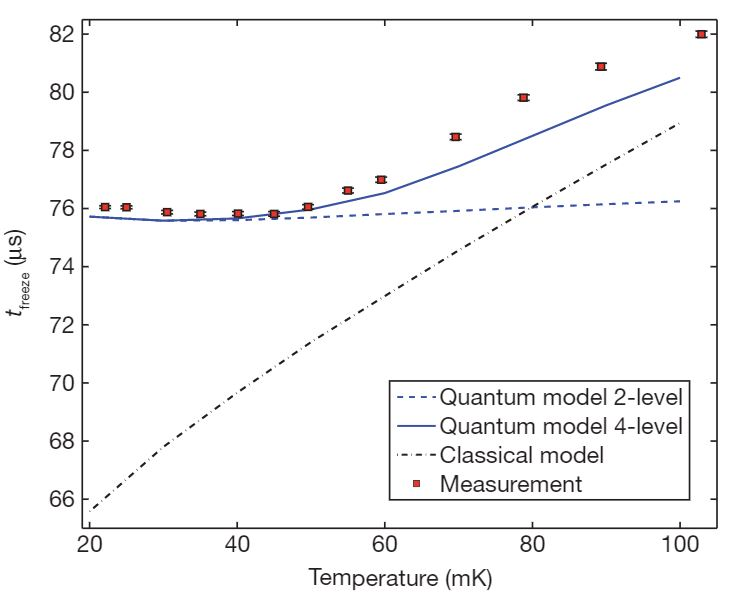
\includegraphics[scale=0.6]{Immagini/qa-chain.jpg}
\caption{Risultati simulazioni per otto qubit.}
\label{figura:qa-chain}
\end{figure}
